\chapter{Related Work}
\label{cha:theory}

This section covers related work done on arrival time prediction 
and motion pattern modeling using spatio-temporal data. It
also covers related work relevant to clustering of trajectory data
and to detection of characteristics in motion patterns.

\section{Arrival Time Prediction}
Arrival time prediction is, in a nutshell, the problem of answering
the question ``When does my bus arrive?''. In recent years, machine learning
techniques have been very successful at this task, and Long Short-Term 
Memory Networks (LSTMs) in particular have proven
extremely effective. J.pang et al. predicted bus arrival times to the next station in a
continuous setting using LSTMs given the current position of a bus and static domain knowledge
about its last stop~\cite{pang2018learning}. 
D. Nguyen et al. also used LSTMs, but with entire
trajectories~\cite{Nguyen2018Jun}. They predicted arrival times of
ships by training a model to generate continuations of trajectories, and  
when the model was presented with a new unfinished trajectory, it generated a
probable continuation until it arrived at a port. This was then used to
make its predictions.

While these approaches do perform admirably on test
data, they lack explainability and a way to measure the models certainty.

\section{Motion Pattern Learning}
Motion pattern learning is the problem of learning motion patterns from a
set of trajectories, such that each pattern captures a different
characteristic of the trajectories. An example with synthetic data can be
seen in Figure~\ref{fig:motion-pattern-example}. Note that the term
\textit{Trajectory learning} is often used in the literature for the
same problem, however, the term ``trajectory'' is ambiguous so in the
scope of this thesis the name motion pattern learning will be used. 
\begin{figure}[H]
  \centering
  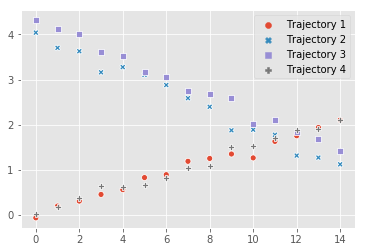
\includegraphics[width=0.7\textwidth]{figures/motion-pattern-example}
  \caption{Synthetic data showing two motion patterns with two trajectories in
    each. Trajectory 2 and 3 belong to one motion pattern and
    Trajectory 1 and 4 belong to a second motion pattern.}\label{fig:motion-pattern-example}
\end{figure}
Motion pattern learning has a natural interpretation as a
clustering problem, but clustering trajectories is difficult,
since different trajectories can have different lengths.
This means that they do not exist in the same vector space and are not
naturally comparable using similarity metrics based on Euclidan
distance. Because of this, more
advanced similarity metrics need to be used. Several different
approaches have been explored, mainly divided by being either deterministic
or probabilistic. Common deterministic techniques
include using spectral clustering with Dynamic Time Warping
(DTW)~\cite{Tang2018Aug} or Longest
Common Subsequence (LCSS)~\cite{Vlachos2002Feb} as similarity metrics.
These similarity metrics are however computationally expensive, making them unsuitable for
real time processing~\cite{Zhang2006Aug}.

\subsection{Probabilistic Approaches}
The probabilistic approach instead fits a model to each motion pattern
and infers its parameters from data. Two popular approaches for this
is fitting Gaussian processes (GPs) and hierarchical Bayesian modeling

\subsubsection{Gaussian Processes}
GPs have been used in several domains for modeling trajectories.
M. Pimentel et al. used GPs to model the vital signs of patients~\cite{Pimentel2013Sep}, 
and were successfully able to cluster the data using hierarchical clustering
and the GP model likelihoods. They then modeled the motion pattern
for a cluster as a GP with the average mean and variance for all GPs in it.
K. Kim. et al. used GPs to model the motion patterns of cars from
surveillance camera~\cite{Kim2011Nov}. They introduce the 
concept of a \textit{frame}, in which the trajectories are
discretisised before fitting GPs to them. Having discrete trajectories meant that
the local likelihood for observed data $x_t, y_t$ in time step $t$
could be computed as $P(y_t | x_t, {M_k})$ for model $M_k$, which
were aggregated to compute a global similarity metric $L_k$,
which in turn was used to cluster the trajectories. To compute the motion
patterns of clusters, a sampling scheme was used. In each time
point, three GPs were drawn uniformly without replacement from the
cluster. The mean value of all drawn GPs were then used as data points
to fit a GP for the clusters motion pattern.

Q. Tran and J. Firl used data with both spatial position and velocity,
and used GPs to model a vector field for each observed
trajectory~\cite{Tran2014Jun}. Before GPs were trained, the trajectories 
were normalised using spline interpolation and a
sampling scheme. They did not perform any clustering. Instead, they
constructed their motion patterns by driving their own test vehicle. 
When presented with a new trajectory, the model could then compute the most
likely motion pattern, and then use a particle filter for the vector
field to predict continuations of motion patterns.

The work of M. Tiger and F. Heintz aimed to improve upon the approach of K. Kim et
al. who had implicitly assumed that all trajectories were generated
from one underlying processes, while a more accurate model is
that they are generated from several different, but dependent
processes. Assuming a single underlying process causes the model to
underestimate its variance, which in turn causes the models likelihood
to be too small for data that is still fairly close.
They aggregated clustered GPs by considering the mixture of
Gaussian distributions they form in a ``slice'', orthogonal to
progression. These slices were then combined to form a single Gaussian
distribution. They then generated synthetic data and learned
hyperparameters for a single GP to approximate the combined Gaussian
distribution, a process they call ``inverse Gaussian process regression''.

C. Leysen et al. also aim to improve on the work of K. Kim et
al~\cite{Leysen2016Sep}. Instead of fitting a GP to re-sampled trajectories, 
they simply select the trajectory in a cluster which maximises the overall
likelihood of the data points in the cluster. While this is less
ad hoc, their approach still assumes a single underlying function for
all trajectory data, and consequently still underestimates model variance.

\subsubsection{Hierarchical Bayesian Models}
The idea behind Hierarchical Bayesian Models used for trajectory
learning is borrowed from the natural language processing field, where
they are known as topic modeling. Topic modeling are unsupervised
techniques for clustering documents into different topics, and by 
considering spatio-temporal trajectories as documents,
their observations as words, and the motion patterns they belong to as
topics, the same techniques can be used to model motion pattern.  
These models are usually based on Latent Dirichlet Allocation (LDA) or
a generalisation thereof known as Hierarchical Dirichlet Process (HDP)
introduced by Teh et al.~\cite{teh2005sharing}, which are both so called \textit{bag-
of-words}-models. A bag-of-words-model assumes independence between
words in a document, which in the domain of trajectories translates to the
assumption that observed data points are independently drawn.

Both LDA and HDP require a set amount of clusters, which is a great
weakness. Wang et al. proposed a model called \textit{Dual Hierarchical Dirichlet
Process} (Dual-HDP)~\cite{Wang2008Jun}, which improves upon the HDP model
by allowing the model to learn the number of topics and documents from
data. Zhou et al. improved upon HDP and LDA by using Markov random
fields to encode prior beliefs in a model called \textit{Random Field
  Topic} (RFT)~\cite{Zhou2011Jun}.

-- this is more recent but I have not been able to figure this paper out yet--
LC-LDA~\cite{Zou2016Apr}

%~\cite{Campo2017Aug}

% HMM on human writing~\cite{Suzuki2007Oct}

% Gaussian Process regression has been used to model trajectories in
% different domains. Medical domain 

% Gaussian Process regression flow in a frame. Requires synchronised
% trajectories and  There  are  some  limitations  and  avenues  of  improve-
% ments.  First, our approach assumes that the types of nor-mal patterns are defined
% a priori. Secondly, if the trajectory is too sparse, 
% the kurtosis measurements in earlier stages of
% the track can be unstable due to the sensitivity of kurtosis
% in a sparse distribution. Finally, our approach does not rec-
% ognize traffic jams and such patterns would be detected as
% an anomaly. A traffic jam, however, can be represented as a
% step shape function in the normalized(u,v,t)coordinates,
% and we plan to use this method to model traffic jams.~\cite{Kim2011Nov}

% similarities (time, space), differences (no frames)

% \subsection{Trajectory Clustering}

% \subsection{Motion Pattern Modeling}


% \section{Motion Pattern Characteristics Detection}


% The main purpose of this chapter is to make it obvious for
% the reader that the report authors have made an effort to read
% up on related research and other information of relevance for
% the research questions. It is a question of trust. Can I as a
% reader rely on what the authors are saying? If it is obvious
% that the authors know the topic area well and clearly present
% their lessons learned, it raises the perceived quality of the
% entire report.

% After having read the theory chapter it shall be obvious for
% the reader that the research questions are both well
% formulated and relevant.

% The chapter must contain theory of use for the intended
% study, both in terms of technique and method. If a final thesis
% project is about the development of a new search engine for
% a certain application domain, the theory must bring up related
% work on search algorithms and related techniques, but also
% methods for evaluating search engines, including
% performance measures such as precision, accuracy and
% recall.

% The chapter shall be structured thematically, not per author.
% A good approach to making a review of scientific literature
% is to use \emph{Google Scholar} (which also has the useful function
% \emph{Cite}). By iterating between searching for articles and reading
% abstracts to find new terms to guide further searches, it is
% fairly straight forward to locate good and relevant
% information, such as

% Having found a relevant article one can use the function for
% viewing other articles that have cited this particular article,
% and also go through the article’s own reference list. Among
% these articles on can often find other interesting articles and
% thus proceed further.

% It can also be a good idea to consider which sources seem
% most relevant for the problem area at hand. Are there any
% special conference or journal that often occurs one can search
% in more detail in lists of published articles from these venues
% in particular. One can also search for the web sites of
% important authors and investigate what they have published
% in general.

% This chapter is called either \emph{Theory, Related Work}, or
% \emph{Related Research}. Check with your supervisor.


